\documentclass[letter,11pt]{article}

\usepackage[english]{babel}
\usepackage[T1]{fontenc}
%\usepackage[ansinew]{inputenc}
\usepackage{lmodern}	% font definition
\usepackage{verse}
\usepackage{datetime}
\usepackage{verbatim}

\usepackage{parskip}
\usepackage{graphicx}
\usepackage[top=1.5cm,bottom=2.5cm,right=1.5cm,left=1.5cm]{geometry}
\usepackage{pdflscape}
\usepackage[numbers]{natbib}
\usepackage{minitoc}

\usepackage[urw-garamond]{mathdesign}

\usepackage{dot2texi}
\usepackage{tikz}

%%%<
%\usepackage{verbatim}
%\usepackage[active,tightpage]{preview}
%\PreviewEnvironment{tikzpicture}
%\setlength\PreviewBorder{5pt}%
%%%>

\usetikzlibrary{arrows,shapes}

\usepackage{url}
\usepackage[ps2pdf,breaklinks=true,bookmarks=true,bookmarksopen,bookmarksopenlevel=1,pdfpagelayout=OneColumn,pagebackref=true]{hyperref}
\usepackage{breakurl}
\usepackage{makeidx}
\usepackage[acronym]{glossaries}

\renewcommand*{\backref}[1]{}
\renewcommand*{\backrefalt}[4]{%
  \ifcase #1 %
	  (Not cited.)%
	\or
	  (Cited on page #2.)%
	\else
	  (Cited on pages #2.)%
	\fi
}

\hypersetup{
    bookmarks=true,         % show bookmarks bar?
    unicode=false,          % non-Latin characters in Acrobat’s bookmarks
    pdftoolbar=false,        % show Acrobat’s toolbar?
    pdfmenubar=true,        % show Acrobat’s menu?
    pdffitwindow=true,     % window fit to page when opened
    pdfstartview={FitV},    % fits the width of the page to the window
    pdftitle={Space-TP ETIR},    % title
    pdfauthor={SU GSP10 Space Team},     % author
    pdfsubject={Space},   % subject of the document
    pdfcreator={SU GSP10 Space Team},   % creator of the document
    pdfproducer={David Dalrymple}, % producer of the document
    pdfnewwindow=true,      % links in new window
    colorlinks=true,       % false: boxed links; true: colored links
    linkcolor=blue,          % color of internal links
    citecolor=green,        % color of links to bibliography
    filecolor=magenta,      % color of file links
    urlcolor=cyan           % color of external links
}

\newcommand{\attrib}[1]{\nopagebreak{\raggedleft\footnotesize #1\par}}
\newcommand{\todo}[1]{\textcolor{lightgray}{\textit{<<#1>>}}}
\newcommand{\tbc}{\begin{center} \todo{to be completed} \end{center}}
\newcommand{\tbcsubsubsection}[1]{ \refstepcounter{subsubsection}%
  \subsubsection*{\thesubsubsection \quad #1} \tbc}
\newcommand{\newacronymd}[3]{\newglossaryentry{#1}{type=\acronymtype,name={#1},description={#2: #3},text={#1},first={#2 (#1)},plural={#1s},firstplural={#2s (#1s)}}}

\setlength{\parskip}{0.3cm plus3mm minus1mm}
\setlength{\parindent}{0cm}
\newcommand{\isp}{$I_{\rm sp}$}

%%GLOSSARY
\newacronymd{CLLSS}{Closed-Loop Life Support Systems}{are life support systems which reuse 100\% of their waste resources, with the exception of waste energy}
\newacronymd{COSPAR}{Committee on Space Research}{COSPAR promotes international scientific research in space, and provides an open forum for the disucssion of problems related to space science (for instance, organizing conferences on planetary protection policy).}
\newacronym{LEO}{LEO}{Low Earth Orbit}
\newacronymd{SSTO}{Single Stage to Orbit}{refers to a vehicle which reaches orbit without jettisoning hardware, expending only fluids. The term usually, but not exclusively, refers to reusable vehicles. \nopostdesc}
\newacronymd{ITAR}{International Traffic in Arms Regulations}{a set of United States federal regulations that restrict the international trade of items and information which is considered by the federal government to be ``munitions,'' including encryption technology and space technology}
\newacronymd{ISRU}{In-Situ Resource Utilization}{refers to the usage of local resources, especially the local usage of resources found in space, as opposed to the transport of Earth resources into space or vice versa. \nopostdesc}
\newacronym{SLS}{SLS}{Selective Laser Sintering}
\newacronym{EBFF}{EBFF}{Electron Beam Freeform Fabrication}

\newglossaryentry{Isp}{text={\isp}, name={specific impulse (\isp)}, first={specific impulse (\isp)}, description={is a metric of rocket (or jet) efficiency; the change in momentum per unit amount of propellant used. (This works out to an SI unit of seconds.) The higher the specific impulse, the less propellant is needed to gain a given amount of momentum. For example, the Space Shuttle Main Engine has an \isp of 453s. \nopostdesc}}
\newglossaryentry{gyrotron}{text={gyrotron}, name={gyrotron}, description={a type of high-powered microwave transmitter}}
\glossarystyle{list}
\makeglossaries
%%END GLOSSARY
% rubber: rules rubber.ini
% rubber: onchange etir.glo '''makeglossaries etir'''
% rubber: watch etir.glo
% rubber: depend etir.glo
% rubber: clean etir.glg
% rubber: clean etir.glo
% rubber: clean etir.gls
% rubber: clean etir.ist
% rubber: clean etir.out
% rubber: clean etir.tdo

\makeindex

\begin{document}

\thispagestyle{empty}
\pdfbookmark[1]{Title Page}{titlepage}
\begin{tikzpicture}[overlay,remember picture]
	\node[yshift=1.5cm] at (current page.center) { 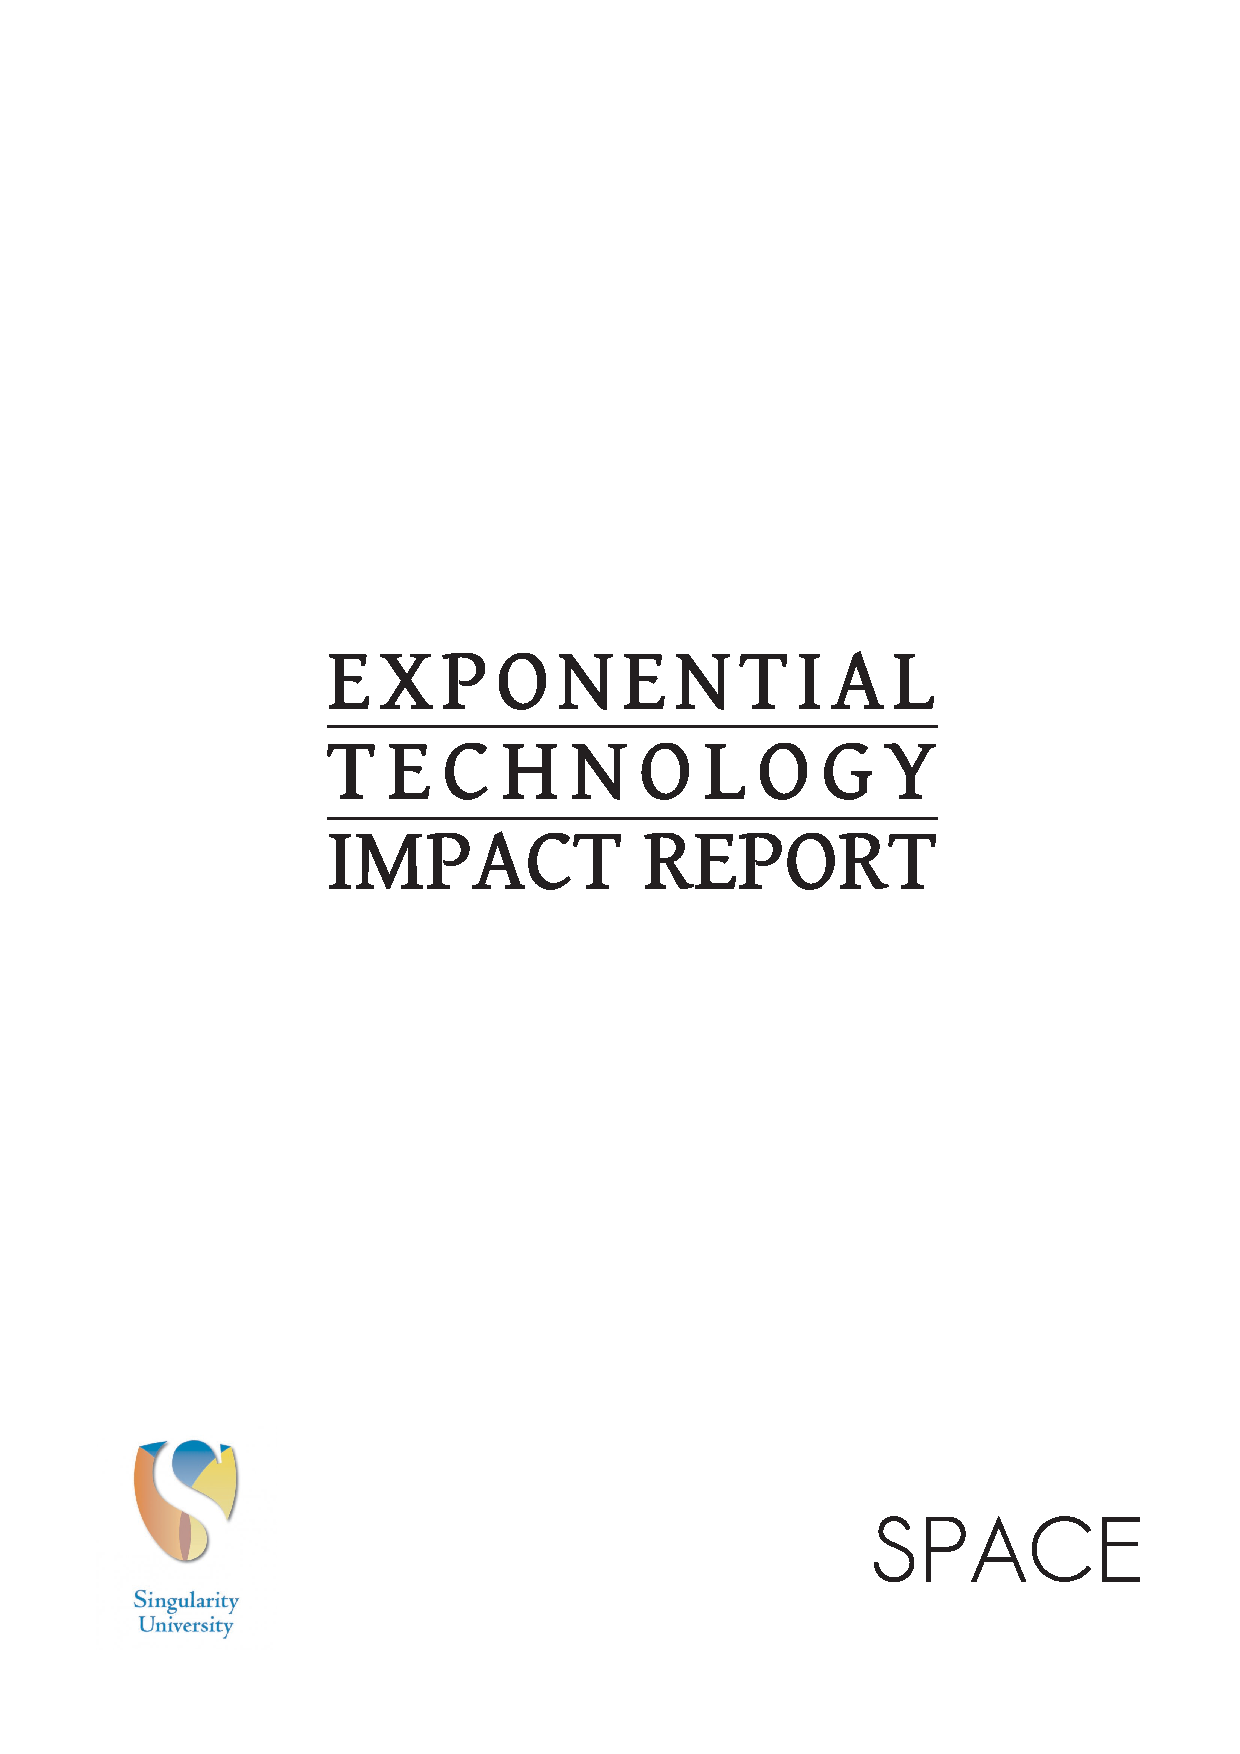
\includegraphics{etir-page1} };
	\node[yshift=0.3cm] at (current page.center) { \huge version 0.foobar };
	\node[yshift=-0.6cm] at (current page.center) { \LARGE \today \hspace{0.2cm} \currenttime };
	\node[yshift=1.2cm] at (current page.center) { \huge \color{red!70!white} \em DRAFT };
\end{tikzpicture}

\newpage
\pdfbookmark[1]{Table of Contents}{contents}
\dosecttoc
\renewcommand{\stctitle}{Contents of this Section}
\tableofcontents

\newpage

\section{Scope of this Report}

\vspace{15pt}
\settowidth{\versewidth}{The surface of the earth is the shore}
\begin{verse}[\versewidth]
	\begin{altverse}
		\em
		The surface of the Earth \\
		is the shore of the cosmic ocean \\
		Recently we've waded a little way up \\
		and the water seems inviting \\
	\end{altverse}
\end{verse}
\attrib{\textbf{-- Carl Sagan\index{Sagan, Carl}}, \textit{``A Glorious Dawn''}}
\vspace{20pt}

Humanity is presently a one-planet species. Although we have sent
humans into space, and even to the moon, they have only visited and
then returned home to Earth. There are two ways in which this
fundamentally limits us: First, it limits the resources available to
us, in terms of both matter and energy. Second, it makes us vulnerable
to total destruction as a species, should a catastrophe of planetary
scale occur.

This report focuses on applications of exponential technologies that may
facilitate the eventual establishment of a permanent human presence in space.
These steps include the development of technologies to reduce the barriers to
entry into space, technologies that may be needed to remain in space
indefinitely (while also being useful on Earth), practical strategies to use
resources which are off Earth, transformative changes in the business of space
science and exploration, and means to educate, excite, and inspire the general
public about the possibilities and importance of human space exploration.

\subsection{Structure of this Report}

\todo{TODO: Graphical diagram explaining structure of final report}

\todo{This part of the document is under heavy construction. This is the temporary home of the digraph.}

\subsubsection{Digraph}

\todo{This is incomplete, represents scope}

\todo{Example about how to parse this graph---narrative threads run bottom-to-top}

\begin{center}
\begin{tikzpicture}[scale=0.41,>=stealth]
	\tikzstyle{stdbox} = [draw,shape=rectangle,minimum size=1em,inner xsep=0.25em,inner ysep=0.25em,font=\footnotesize,text badly centered];
	\tikzstyle{emph} = [font=\small\bfseries,very thick];
	\colorlet{challenge}{red}
	\colorlet{exptech}{green}
	\tikzstyle{challenge} = [stdbox,draw=challenge,emph,fill=challenge!50];
	\tikzstyle{exptech} = [stdbox,draw=exptech,emph,fill=exptech!50];
\begin{dot2tex}[codeonly,dot,tikz]
digraph G {
  ratio=1.2;
	rankdir=BT;
	//% GRAND CHALLENGES
	node [style="challenge"];
	getting_there [label="Getting There"];
	staying_there [label="Staying There"];
	human_exploration [label="Human Exploration",style="challenge,xshift=0.4cm"];
	resources [label="Space Resources"];
	robotic_exploration [label="Robotic Exploration",style="challenge,xshift=0.2cm"];
	science [label="Space Science"];
	education [label="Space Evangelism"];
	backup [label="Insuring Humanity"];

	edge [style="thick,color=challenge"];
	human_exploration -> staying_there; //[dir="none"];
	robotic_exploration -> science;
	robotic_exploration -> resources;
	staying_there -> backup; //[dir="none"];

	edge [style="semithick,color=challenge!70!black"];
	resources -> staying_there; //[dir="none"];
  getting_there -> resources;
	human_exploration -> science; //[dir="none"];
	getting_there -> education;
	getting_there -> robotic_exploration;
	getting_there -> human_exploration;

  //% EXPONENTIAL TECHNOLOGIES
	node [style="exptech"];
	nano [label="Nanotechnology"];
	bio [label="Biotechnology"];
	neuro [label="Neurotechnology"];
	ai [label="AI & Robotics"];
	computing [label="Networks & Computing"];

	edge [style="thick,color=exptech"];
	computing -> ai;
	neuro -> ai [dir="both"];
	computing -> bio;
	ai -> bio;
	bio -> nano;
	bio -> neuro;
	nano -> computing;

  node [texmode="raw",style="stdbox"];
	edge [style=semithick];
  cats [label="CATS"];
	cats -> getting_there;
	beam_power [label="Beam Power"];
	beam_power -> cats;
	heat_exchanger -> beam_power;
	heat_exchanger [label="Heat Exchanger"];
	structural_materials [label="Structural Materials"];
	thermal_materials [label="Thermal Materials"];
	nano -> thermal_materials;
	nano -> structural_materials;
	thermal_materials -> heat_exchanger;
  structural_materials -> light_lv;
	light_lv [label="Lighter Launch Vehicles"];
	light_lv -> cats;
	light_lv -> ssto;
	ssto [label="Single-Stage to Orbit"];
  ssto -> cats;

	psychmon [label="Psych. Monitoring"];
	neuro -> psychmon;
	psychmon -> human_exploration;
	rubisco [label="RubisCO Enzyme"];
	bio -> rubisco;
	terraforming [label="Terraforming"];
	rubisco -> terraforming
	terraforming -> staying_there

	asteroid_mining [label="Asteroid Mining"];
	asteroid_mining -> resources;
	cats -> asteroid_mining;
	metal_digesters [label="Metal Digesters?"];
	bio -> metal_digesters;
	metal_digesters -> asteroid_mining;

	auto_asteroid [label="Autonomous Asteroid Explorers",style="stdbox,text width=2.6cm"];
	ai -> auto_asteroid;
	auto_asteroid -> robotic_exploration;
	auto_asteroid -> asteroid_mining;

	ipip [label="Interplanetary Internet"];
	computing -> ipip;
	ipip -> auto_asteroid;
	//ipip -> space_science;

	spider_silk [label="Spider Silk"];
	spider_silk -> structural_materials;
	bio -> spider_silk;
	stem_cell_min [label="Stem Cell Anti-Demineralisation",style="stdbox,text width=2.6cm"];
	bio -> stem_cell_min;
	stem_cell_min -> human_exploration;
	bioreactors [label="Bioreactors"];
	bioreactors -> terraforming;
	bio -> bioreactors;
}
\end{dot2tex}
\end{tikzpicture}
\end{center}

\section{State of the Problem Space}

\subsection{Overview}
% Short description of the entire Problem Space

Doing business in space should be easy, but it isn't. It's hard to get into
space, even sending robots rather than humans. It's hard to stay in space for
very long--again, even if you send robots.  It's hard to make use of the
resources available in space. And it's hard to convince many people that going
to space is even a good idea.

\subsection{Aspects}

We have chosen to focus on the following aspects of the problem space:

%NOTE: don't worry about extra spaces which may appear in copy+pasting to and from
%Etherpad. Remove them if they bother you, but otherwise TeX will remove them for you
%when the document is compiled to PDF.

\subsubsection{Getting There}
%(to be written by Dmitriy)

\subsubsection{Staying There}
%(to be written by Eric)



\subsubsection{Human Exploration}
%(to be written by Sarah Jane)

\subsubsection{Robotic Exploration}
%(to be written by Jan)

\subsubsection{Space Resources}
%(to be written by Mike)

\subsubsection{Space Science}
%(to be  written by Diva)

\subsubsection{Space Education/Evangelism}
%(written by Jason, edited by davidad)

A key underlying problem to the limit  of humanity's progress in space is that the majority of the human  species is uninterested in space. Activities in space today do not  inspire the awe that they once did: instead of watching astronauts walk  upon the surface of a celestial body for the first time, today, if we're  lucky, we get to watch them repair the toilet on the International  Space Station. Educational outreach is a good start, but we need to  connect humanity to space in a more natural way. Global warming is now  perceived as a threat so compelling that most people believe we need to  do something about it. But this threat is dwarfed by that of remaining  on this planet indefinitely.

NASA's  education program attempts to make space and the STEM (Science  Technology Engineering and Math) curriculum exciting for students, but  they do it without an understanding of the progress exponential  technologies will have on the space industry. Students today rarely  realize that when they grow older they will have a completely different  tool set with which to tackle space. We should teach them what the world  will be like in a decade or two and excite them on the possibilities  they can create.

In  all instances of educating the public on the importance of space, from  youth to the elderly, opening the space frontier is never presented as  an explicit need---which it is. Space is often considered to be  primarily beneficial as an engine for creating technological spin-offs,  but even if space exploration paid no technological dividends, it would  still be crucially important. People don't appreciate the voyage of  Christopher Columbus to the Americas primarily because of the new  sextant developed for the journey that was eventually spun off to the  private sector and used in merchant shipping.

It is human nature that we need to  "see it to believe it," and maybe this is what is holding back humanity  from understanding why space exploration is a necessity for survival.  Until ordinary people can experience space through their own eyes, the  possibilities that it holds will not be fully understood. What will  happen when the first child can see our home from space, or when the  first ballet dancer experiences weightlessness, or when a paraplegic is  given mobility again? Let's not just tell humanity about space, let's  give them access to space.


\subsubsection{Insuring Humanity}
%(to be  written by davidad)



\begin{comment}
\subsection{Breakdown}
% Detailed description of the aspects of the problem being addressed
\begin{itemize}
	\item \textbf{Getting There/Transportation}: Cheap access to space is the single most important thing that could happen to drive space exploration and colonization \begin{itemize}
			\item Earth to \gls{LEO}: Propulsion systems with higher thrust and \gls{Isp} are needed, \gls{SSTO} vehicles would be ideal, and our current systems are largely non-reusable and made from materials that are highly suboptimal from a theoretical point of view.
			\item \gls{LEO} to Anywhere: Propulsion and braking systems with high \gls{Isp} and low thrust are needed, along with light structure spacecraft, formation flying, radiation shields, etc.
				\item Raw Materials: As all tools and parts used in space are currently made on Earth, they must be made to high tolerances and sent on relatively low-acceleration launch vehicles to prevent damage; shipping raw materials would not have such problems.
				\item People: Space travel is still far riskier than commercial aviation, and there are few mechanisms by which spacecraft can fail while keeping the crew alive.
			\end{itemize}
	\item \textbf{Staying There} \begin{itemize}
			\item \textbf{Research Labs}: Some research is not possible in the Earth's gravity.
			\item \textbf{Permanent coloines} \begin{itemize}
					\item In \gls{LEO}: Need reliable infrastructure and life support
					\item On the Moon: Desire robotics for automated resource extraction, construction and maintenance.
				\end{itemize}
			\item \textbf{Funding/business models}: Need a space-based economy that doesn't rely on Earth (complete \gls{ISRU} for an entire society).
			\item \textbf{Social and political structures}: Ensuring that citizens of space societies are safe and granted basic rights. Negotiations between space colonies and space$\leftrightarrow$Earth.
			\item \textbf{Ownership}: How shall it be decided who owns portions of space, or resources brought back from space?
			\item \textbf{Speciation/Human mutation}: Societies colonizing space for a long period of time will eventually become a different species from those on Earth. This raises many ethical and political issues.
			\item \textbf{Communications}: Need a self-configuring, adaptive deep-space network, tied to the Internet.
			\item \textbf{Universal timestamping}: To enable information exchange, we will need standard ways to timestamp data and standardize metrics for measurement.
			\item \textbf{Resupply}: Need for a cheap launch system, cheap propulsion between the supply station and the colonies, and access to continual resources
			\item \textbf{In-situ resource utilization}: extracting and using resources from planets, moons, and asteroids, for usage in construction, propulsion, power, sustenance for astronauts.  Overall goal is to build systems that sustain, grow, and replicate without input from Earth.
			\item \textbf{Terraforming} \begin{itemize}
					\item Atmosphere: Need to develop an atmosphere with a balance similar to Earth's, allowing life to flourish (proper balance of nitrogen, oxygen, argon, and CO2). Also need to maintain the atmosphere (example: having a magnetosphere on Mars).
					\item Soil: Soil leads to plant life and the consistent production of food. Plant life will lead to an ecosystem on Mars and other celestial bodies that will help maintain the atmosphere and allow life to flourish.
					\item Microbes: How might we synthetically engineer microbes for the purpose of sending them to remote planets and having them perform terraforming processes?  To what extent do we need to be careful about introducing certain lifeforms to remote planets?
				\end{itemize}
		\end{itemize}
  \item \textbf{Robotic Exploration} \begin{itemize}
			\item Remote Controlled: Our current interfaces are insufficiently natural, lacking haptic feedback or immersive views, and deal poorly with low bandwidth and high latency.
			\item Semi-autonomous: The latest space technology lags far behind the state of the art in ``narrow AI'' or planning algorithms.
			\item Fully autonomous: Nearly all space missions today must be heavily monitored and guided from the ground.
			\item Communications: Our communications infrastructure in both near and deep space leaves much to be desired, and cannot support an exponentially growing quantity of space computing nodes.
			\item Better materials: Need materials that are stronger, lighter, and easy to develop/replicate. Weak materials fall apart in space's harsh environments, heavy materials increase transit time, and rare materials limit product line.
		\end{itemize}
	\item \textbf{Human Exploration} \begin{itemize}
			\item \textbf{\gls{CLLSS}} \begin{itemize}
					\item Food: Need for a way to generate a complete, well rounded diet with minimal input and output - ideally 100\% closed loop.
					\item Water: Need for sophisticated waste and grey-water systems for closed-loop water usage.
					\item Waste: Design waste out from the beginning - systems should operate in completely closed loops for matter and energy.
					\item Air: Assure fully closed-loop air systems able to work indefinitely at extreme reliability.
				\end{itemize}
			\item \textbf{Human Health}: Issues include psychological health, crew selection, training, habitability and human factors requirements, social governance supports, infrastructures for long duration spaceflight, consent and justice for one-way missions, and strategies for permanent colonisation with ethical micro- and meso-social structures. \begin{itemize}
					\item Radiation Shielding \begin{itemize}
							\item Need to establish acceptable radiation exposure limits
							\item Need for formal alert/warning and communications infrastructure from pre-screening to initial construction to settlement.
							\item Need mechanical counter-pressure and electrostatically charging materials for suit design.
							\item Need to analyze long-term health risks.
						\end{itemize}
					\item Extreme habitat design: Need for human-rated and ``homey'' design, including spaces for privacy and socialisation, localized vehicles, sick bays, architecture with built-in physical countermeasures, teleconferencing/VR, hydrotherapy, color and light, and views of Earth, if possible. Also, new materials technologies are desirable, including: \begin{itemize} \item inflatables \item demountables \item transformers \item smart materials \end{itemize}
					\item Psychological well-being: Space radiation poses poorly understood risks to the central nervous system. Besides the late effects of long term radiation exposure, stress, deprivation, isolation, and confinement constitute major risks for the physical and mental health of space explorers during the missions.
					\item Pharmacological support: treating space-related osteoporosis, cardiovascular problems, vitamin and nutrient loss, sleep disturbance, muscle atrophy, and cellular damage
				\end{itemize}
		\end{itemize}
	\item \textbf{Using Space Resources} \begin{itemize}
			\item \textbf{Energy Harvesting and Beaming}: Need a way to harvest resources and energy from the massive array of sources available in space. Asteroids and solar are likely the two most impactful.  As far as beaming goes, a system is needed to transmit the energy from space to the ground.  In the case of asteroids, transport of physical resources is needed.
			\item \textbf{Asteroid Mining}: Need a cost-effective way to reach near-earth asteroids, and a means to map, identify and choose which to go to. Also, desire automated mining techniques, self-replicating robots for networked mining swarms, mesh networks, autonomous behavior, and 3D printing for tool generation and maintenance
			\item \textbf{Political Challenges} \begin{itemize}
					\item Security restrictions such as \gls{ITAR}: Need a framework for international cooperation in the private sector
					\item Space treaties:  Need \gls{COSPAR} regulations - sample return restrictions and planetary protection guidelines. There is some international disagreement.
					\item Fueling: Need for an international agreement that takes into consideration peaceful use, human safety, and waste mechanisms related to the extraction and utilization of fuel and nuclear energy
					\item Real Estate: No state has a claim to land rights in space; can private entities?
					\item Public/private partnerships: Need to exploit the full potential of spin-in and spin-off technologies. Space is more closed than other sectors. There are also underdeveloped marketing opportunities.
				\end{itemize}
		\end{itemize}
	\item \textbf{Education/Space Evangelism}: We need to enable the world to learn about space in awe-inspiring new ways. Most people don't want to be ``taught,'' so the focus of the education problem is fostering excitement, enabling people to learn on their own, and showing people that we're all connected to space.
\end{itemize}
\end{comment}

%\subsection{State of the Art}

\subsection{Exponential Technology Areas}
% Summary list\ldotsof what you considered, based on the SU tracks, for example

In this report, we will illustrate a number of opportunities to address the
above problems with exponential technologies. This section serves as a brief
overview to each of the exponential technology areas.

\subsubsection{AI and Robotics}

% [Can we make this paragraph a vision statement rather than a historical statement?
% Something more from http://su-etherpad.com/tpspace-The-Real-New-Space ?]
%   [davidad: this is intended to be a historical orientation, but feel free to add a
%    third paragraph that is more visionary in tone.]

In the broadest sense, the fields of AI and robotics strive to make non-human systems able to perform human tasks%
%Is this too limiting a view of AI and robotics? -- Will they just be worker tools, or the
%beginnings of a future of extraordinary intelligence and physical capabilities?)
, or other difficult tasks that are helpful to humans. Robotics focuses on the necessary physical capabilities, while AI focuses on the necessary mental capabilities. At present, AI systems are capable of solving a plethora of individual problems, each of them far more swiftly and accurately than a human could; but no robot is capable of loading a dishwasher yet.
% I would not make this point, as Robots already wash our dishes today far better than
% humans do (including total disinfection), and don't do it at all the way we do (contained
% machines). Planes also don't fly like birds, but we might say they are far better for our
% purposes.
This phenomenon is represented by the term "narrow AI": each AI system today is typically helpless outside the situation it was designed for. These systems solve problems such as searching the Internet, routing FedEx packages, military logistics, or playing chess. However, it has been predicted that in the future, we wil develop what is known as "strong AI": an AI system that nears human levels of tolerating uncertainty, and can generate original solutions to problems hitherto unseen and unanticipated by the designers of the AI.

\subsubsection{Biotechnology}



\subsubsection{Nanotechnology and Materials Science}



\subsubsection{Information Technology and Networking}



\subsubsection{Neurotechnology and Medicine}



\subsubsection{Policy, Law, and Ethics}

We are not in a position to fully analyze the far-reaching consequences of near-term steps by space agencies and private space entrepreneurs, however we can set about to establish a  context for critical evaluation of our motivations and hesitations at the Singularity University during the 2010 GSP. This is a time to develop a culture of intense questioning and reflexivity, weighing up the pros and cons of social and education value, economic and political drivers, scientific benefits, risks, the battle for sovereignty between nation states; time readiness, and the lessons learnt from past human endeavors at each stage of mission  planning and undertaking. Particular attention must be paid to our obligations and restrictions, the differences of moral standing and the agents behind them; the intrinsic and instrumental values of global peoples and the core truths of our calling, in order to plan effectively and to garner new insights and knowledge for wider reaching solutions to terrestrial concerns so that we can leverage exponentially advancing technologies for the benefit of humanity, the planet and the future of our activities in space. We have a responsibility to boldly stay to serve legitimate interests as a peaceful, well-meaning people and the opportunity to explore new ways of seeing life, and space, from a whole new perspective. 

It is posited that if we are to actually improve standards of living on Earth through space by  generating economic opportunity; providing access to new resources (material, intellectual and so on) then we need to bring about the prospect of rapid technological development, the cross-fertilization of ideas, new visions and shared dreams for the benefit of all human-kind and this begins with the power of the questions we ask ourselves, and the declarations we make for our future generations. 

\subsubsection{Entrepreneurship}



\subsection{Classification of opportunities}

We offer a brief taxonomy of the problems that exponential technologies need to
help overcome during the next three decades in order to facilitate the
exploration and colonization of space. For each area in this taxonomy, we
explore the role that each exponential technology might play.

\begin{enumerate}
	\item AI and Robotics \item   Biotechnology \item  Nanotechnology and Material Sciences \item  Information Technology and Networking \item  Neurotechnology and Medicine \item  Policy, Law and Ethics \item Entrepreneurship 
\end{enumerate}

The goal of these definitions is twofold: to map for future reference
our current understanding of the relative role of each of the
exponential technologies and solution domains, and to help us focus our
in-depth analysis of conceptual solutions to those areas that appear
more fruitful.

\begin{comment}
We have divided the problem space in two different ways, which we call {\em heatmaps} and {\em roadmaps}. First, we have
intersected each of the problem areas in section 2.2 with each of the
exponential technologies in the above outline. Second, we have focused on
30-year roadmaps for each exponential technology, and intersected the roadmaps
with aspects of the space exploration problem. (Unfortunately, the latter
roadmaps are in a form that is not easily converted to the printed page; a
later version of this report will contain a visualization of these roadmaps.)
The qualitative analysis of the relative importance of each of the solution
domains is presented in the form of a series of \emph{heatmaps}, according to
the following scale:\newline

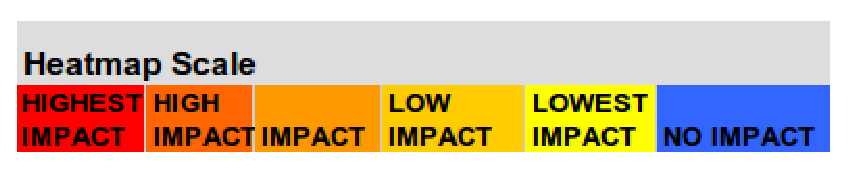
\includegraphics[width=4.2in]{Heatmapscale}
\newline

\newpage

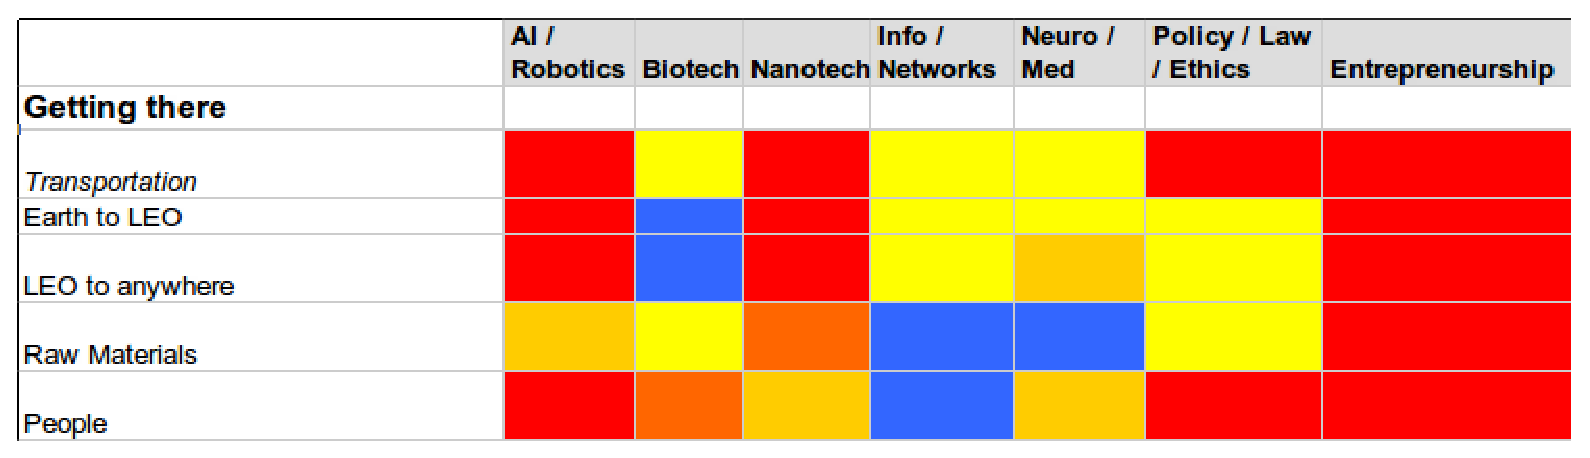
\includegraphics[width=\textwidth]{hm_gt}
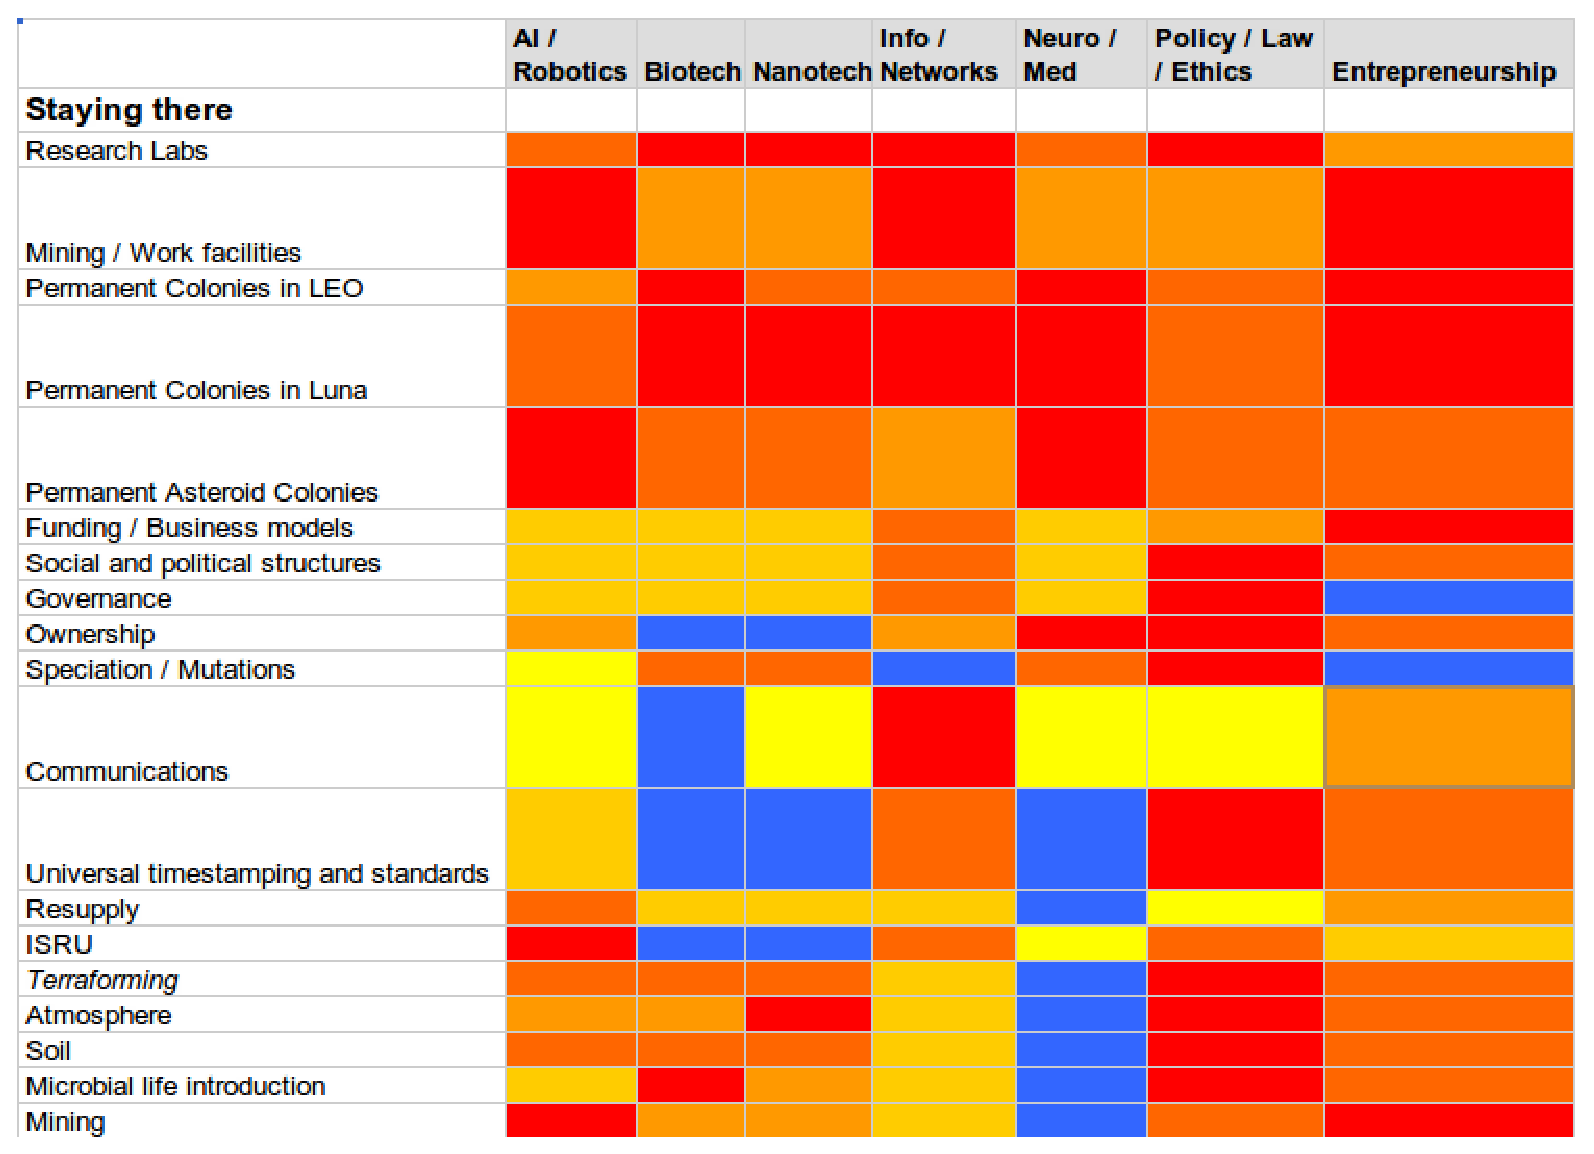
\includegraphics[width=\textwidth]{hm_st}
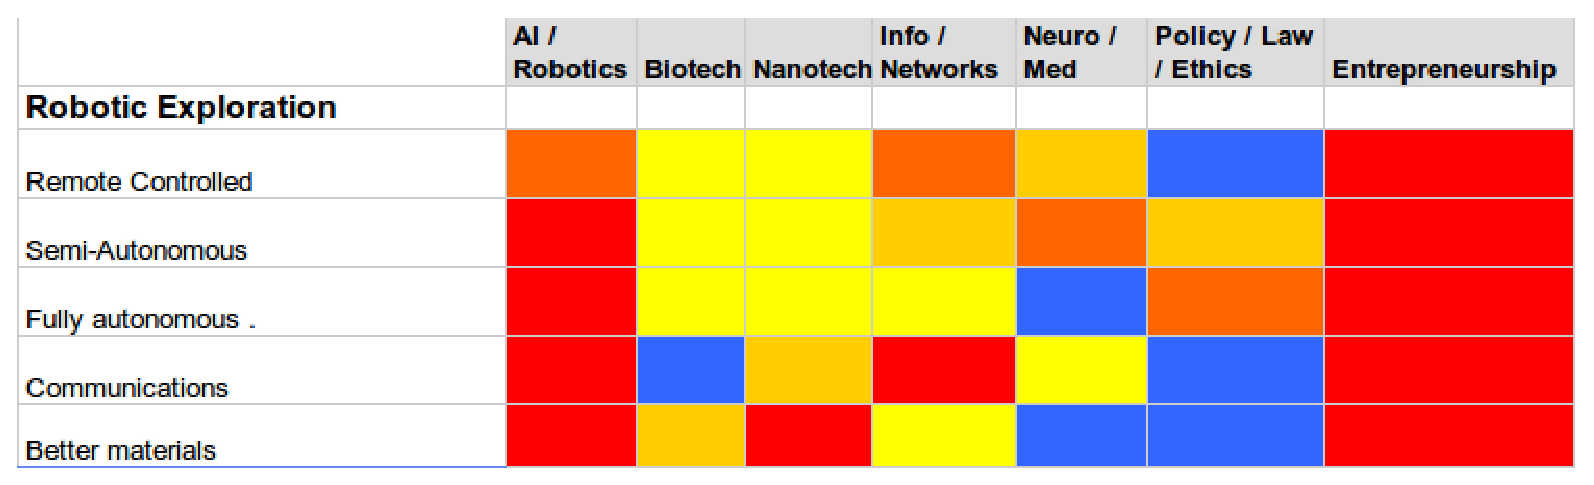
\includegraphics[width=\textwidth]{hm_re}
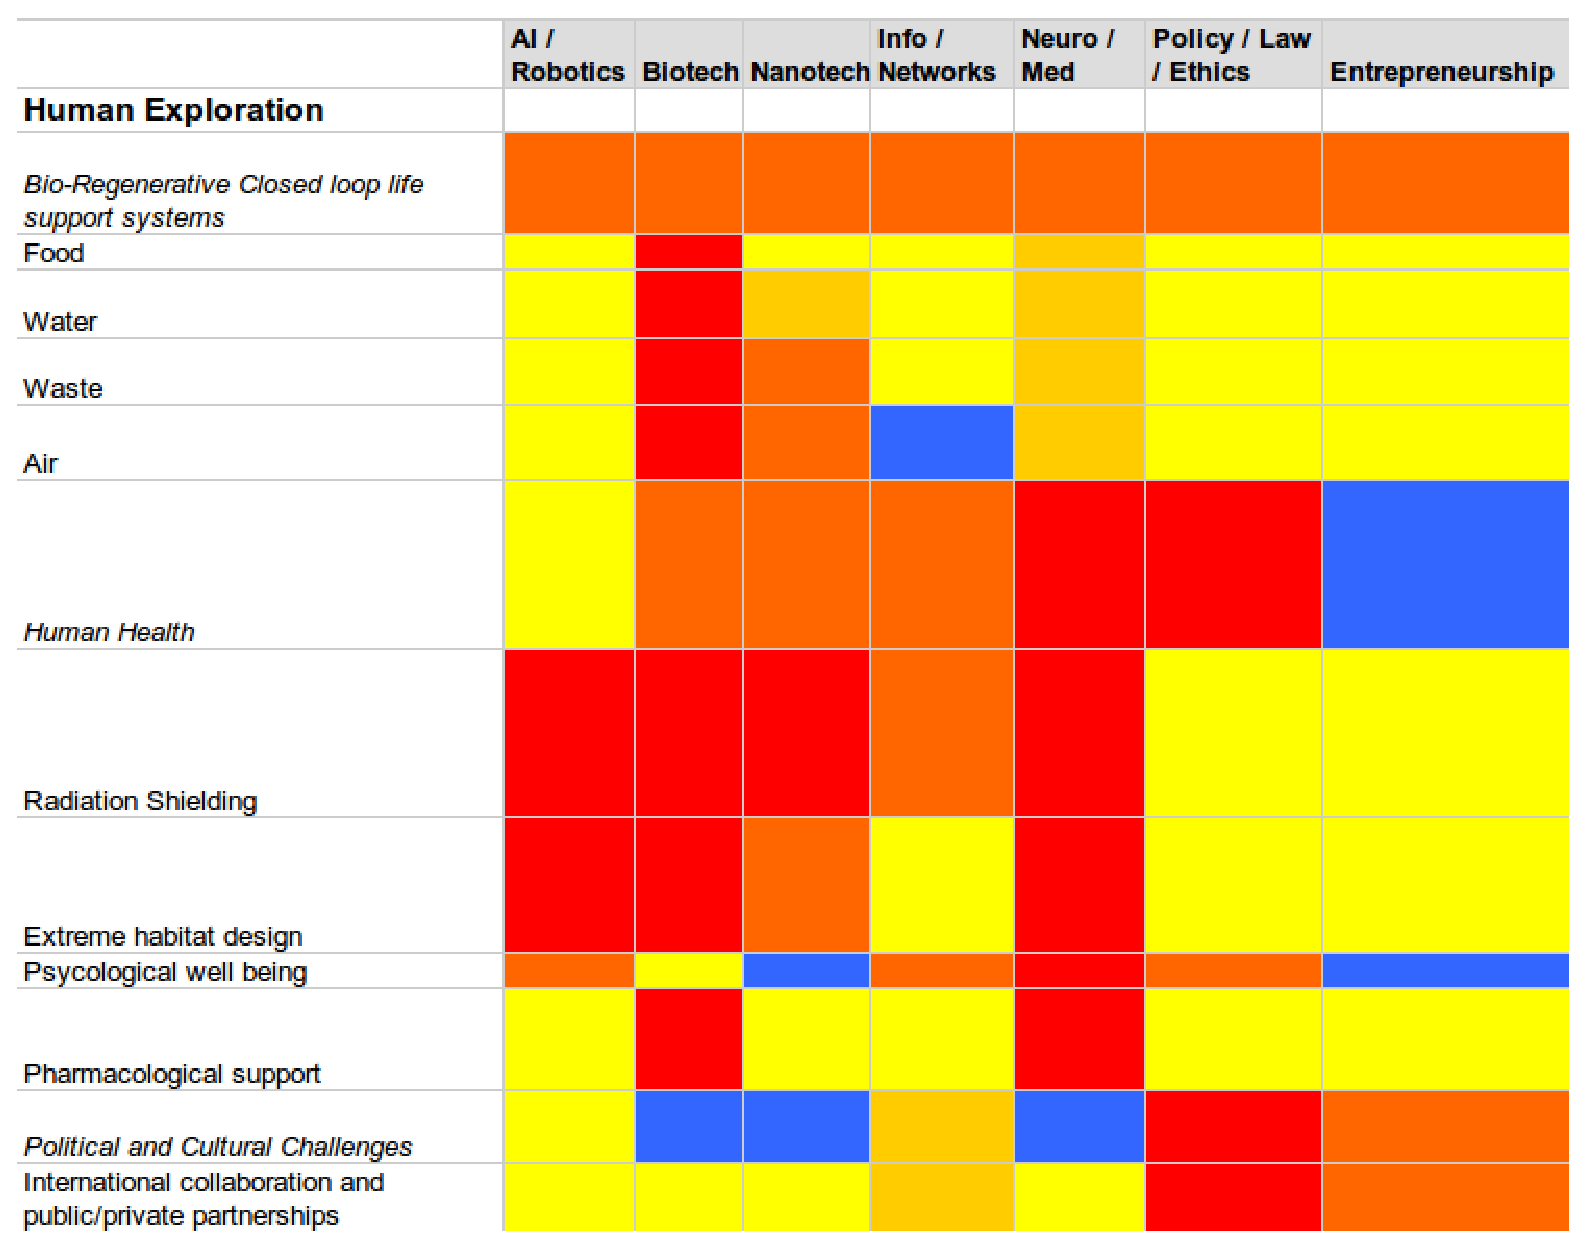
\includegraphics[width=\textwidth]{hm_he}
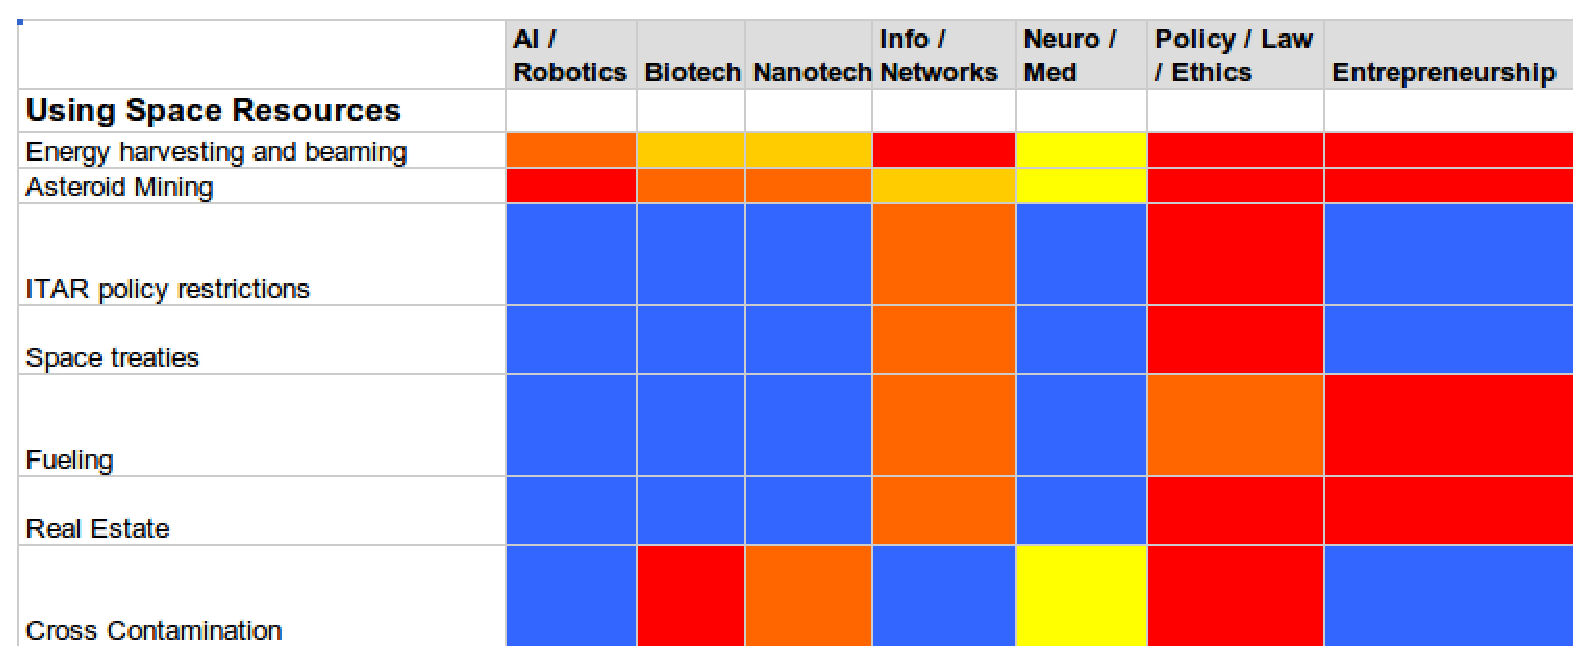
\includegraphics[width=\textwidth]{hm_usr}

\includegraphics[width=\textwidth]{hm_e}
\end{comment}

\section{Exponential Technology Opportunities}

$\ldots$For each of the sections below, we discuss the current state of the art,
related exponential technologies, potential benefits, convergences with other
technologies, and potential barriers to adoption.

\secttoc

\begin{comment}
	All these sections will be replaced by Chrisographs...
\subsection{3D Printing in Space}

Tools and parts for space exploration must be comprehensive, redundant,
and able to withstand the forces of launch. As a result, they are bulky
and inconvenient, and despite this, situations still occur in space when
the right tool for the job is simply not available. New 3D printing
technologies can change that. The future lies with fast, customizable
manufacturing, with which tools and parts can be built on-demand in space.

\subsubsection{State of the Art}
% assess the current state of the technology
% identify companies, researchers, etc working in this area, with links and references

Today's 3D printers here on Earth can fabricate objects made of some metals,
ceramics, and plastics, and the palette of materials is expanding
exponentially.  There is even one 3D printer currently in production which can
print objects made of more than one material. However, most current 3D printing
mechanisms will not work in microgravity environments. For example, \gls*{SLS}
uses a laser to selectively fuse together particles of build material (be it
metal, ceramic, or plastic), building up the object layer-by-layer by a process
of powder deposition. Without gravity, such deposition is impossible. A new
technique called \gls*{EBFF} \cite{Taminger2006}
pioneered at NASA Langley overcomes this challenge by extruding metal directly
from a tip. This is a promising technology, but is currently too heavy and
low-resolution to be practically useful in space.  However, these are merely
problems of engineering that will improve with the exponential increase in the
strength of materials.

\subsubsection{Related Exponential Technologies}

\begin{itemize}
  \item Networks and computing systems enable the digital shipment of high-resolution
part files \\
  \item AI can automate the process of designing a tool or choosing a tool design,
given information such as a 3D scan of a machine to be repaired \\ \item Nanotechnology will result in more precise fabrication processes, less waste of
materials, and more easily reusable materials (i.e. nanodisassembler)
\end{itemize}

\subsubsection{Potential Benefits}
% make an estimate of the potential benefit of this technology
% estimate if this is near term or longer term, or other labels to measure the opportunity

In the near term, the greatest use of 3D printing in human space missions is printing tools or components as they are needed. Custom-built tools mean fewer tools taken to orbit with less redundancy in number of tools taken. In the longer term, 3D printers are compelling and enabling tools for human colonization. The ability of either robots or humans to be able to print what is necessary using local materials is a compelling reason to pursue this technology.

\tbcsubsubsection{Convergences}
% identify if there is a convergence (or mutual benefit) from other technologies

\tbcsubsubsection{Barriers}
% identify potential barriers to the development or adoption of this technology
% identify significant bottlenecks in technology, process, law, policy, regulation, and approaches and potential solutions to these bottlenecks (this detailed assessment would be applied to opportunities you chose to highlight)

\subsection{Asteroid Mining}

There are not enough raw materials present on planet Earth to sustain even
today's level of technological growth for the next 20 years\cite{Cohen2007}.
Perhaps even more astonishingly, there are not even enough raw materials on the
planet for the world's current population to live with the quality of life of
the modern developed world\cite{Gordon2006}.  Thankfully, while these raw
materials are scarce on Earth, they are highly abundant in the numerous
near-Earth asteroids and comets that circulate our solar system.  Hence, it is
of great importance that a powerful initiative be put in to place to secure the
valuable materials from these bodies and bring them back to Earth.

\tbcsubsubsection{State of the Art}
% assess the current state of the technology
% identify companies, researchers, etc working in this area, with links and references

\subsubsection{Related Exponential Technologies}
\begin{itemize}
	\item As artificial intelligence and computing increase exponentially in
		power, the degree of autonomy that is available for robotic mining of
		remote asteroids will grow powerfully, enabling cheaper and more successful
		missions
	\item Advances in biotechnology will enable us to engineer synthetic
		organisms that extract and refine materials from asteroids cheaply and
		reliably
	\item As our networks and communications systems become more capable, so will
		our ability to communicate with remote mining systems and colonies
	\item The availability of nano-satellites will enable cheap, small, and
		highly redundant mining missions to numerous asteroids in our solar system
\end{itemize}

\subsubsection{Potential Benefits}
% make an estimate of the potential benefit of this technology
% estimate if this is near term or longer term, or other labels to measure the opportunity

Mining the asteroids will not only avert the global crisis that would have been
brought about by a poverty of critical resources, it will usher in a new era of
utopian abundance in the near-term future of humankind.

\tbcsubsubsection{Convergences}
% identify if there is a convergence (or mutual benefit) from other technologies

\subsubsection{Barriers}
% identify potential barriers to the development or adoption of this technology
% identify significant bottlenecks in technology, process, law, policy, regulation, and approaches and potential solutions to these bottlenecks (this detailed assessment would be applied to opportunities you chose to highlight)

The successful return of asteroidal resources to Earth presents a number of
deep challenges.  It is quite likely that such a success would be preceded by a
series of unsuccessful attempts, rendering the ultimate success prohibitavely
expensive.  In this section, we \todo{will} describe a set of paradigm-shifting
asteroid mining methods that are made possible by the great wealth of powerful
exponentially growing technologies that will be available in the next 10 to 20
years.

\subsection{Beam Power}

\subsubsection{State of the Art}
% assess the current state of the technology
% identify companies, researchers, etc working in this area, with links and references

Since the first rocket launch, the cost of launching objects into space has
never dropped exponentially.  This has been a major impediment to the
advancement of the space industry, and many exponential industries such as the
computing industry have left it behind in the dust.  Perhaps the most promising
way to turn space launch into a technology that decreases in price
exponentially is external propulsion. In such a system, instead of carrying
both fuel and propellant onboard the launch vehicle, the energy to exhaust the
propellant is provided from outside the vehicle, for instance via a microwave
beam, and transduced into thrust by a heat exchange engine. An externally
powered space launch system represents a completely new paradigm of space
access as it transfers all of the expensive and heavy components associated
with the space launch to the ground facility and opens an opportunity for the
design of highly efficient and cheap launch vehicles. Once the ground facility
is established, the cost of space launch can be reduced essentially to the cost
of associated resources, such as energy delivered from the ground and hydrogen
propellant.

\subsubsection{Related Exponential Technologies}

The microwave system will decrease in price as the price per megawatt decreases
over time.  This price will decrease over time as the maximum power output of
each individual \gls{gyrotron} increases over time, and the cost of each
gyrotron decreases over time.  The maximum power output of each individual
gyroton will increase over time as superconductor performance increases and as
computing power increases, insofar as computing power influences the control
dynamical systems in the gyrotron.  Gyrotons will get cheaper as the 3D
printing of materials gets cheaper over time and 3D printing technology
increases in capability.  Also, the gyroton cost will decrease as
superconductors get cheaper and more effective.  The materials required for the
diamond window component will also decrease over time.  Control dynamical
systems will become cheaper as computing power gets cheaper and also as 3D
printing gets cheaper and more effective.

The heat exchange engine will get cheaper as the turbopump gets cheaper, which
will primarily be driven by 3D printing getting cheaper and more effective.
The hydrogen tank component of the heat exchange engine will get cheaper as the
manufacturing of nanocomposite materials becomes more effective.  This will be
driven precisely by the decrease in the mass of the tank and the decrease in
the price of the tank, while the volume and strength of the tank are held
constant.  The heat exchanger component of the engine will become cheaper as
the manufacturing of nanocomposite materials becomes more effective and cheaper
over time.

The launch vehicle itself will become cheaper as well as the manufacturing of
nanocomposites becomes more effective and cheaper, and as the mass of the
launch vehicle decreases while the strength of its structure remains constant
over time.

Finally, preflight testing and design will become cheaper as computer-aided
design becomes more effective and cheaper, which will happen as computing power
becomes more powerful and cheaper, and as CAD algorithms improve.  Preflight
testing and design will also beome cheaper as multiphysics simulations become
more powerful.  This will be a result of software functionality improving,
hardware functionality improving, crowd-sourcing more prevalent, and regulation
becoming more slack on the levels to which technology must be tested.

\subsubsection{Potential Benefits}
% make an estimate of the potential benefit of this technology
% estimate if this is near term or longer term, or other labels to measure the opportunity
The microwave beam-powered launch system will decrease in price exponentially as a result of four of its components decreasing in price exponentially. In addition, we expect the following benefits:
\begin{enumerate}
	\item Single Stage to Orbit with an increased safety factor and full reusability
	\item 5--10 times more payload into orbit than a chemical rocket of the same initial mass
	\item One type of propellant, no chemical reactions on board
	\item Much simpler, highly modular launch vehicle with cheaper construction and maintenance
\end{enumerate}

\tbcsubsubsection{Convergences}
% identify if there is a convergence (or mutual benefit) from other technologies

\tbcsubsubsection{Barriers}
% identify potential barriers to the development or adoption of this technology
% identify significant bottlenecks in technology, process, law, policy, regulation, and approaches and potential solutions to these bottlenecks (this detailed assessment would be applied to opportunities you chose to highlight)

\subsection{Biology-Based Life Support Systems}

\subsubsection{State of the Art}
% assess the current state of the technology
% identify companies, researchers, etc working in this area, with links and references
Identifying mineral biomarkers used for the search for life in space. Discovery of microbial habitability in air (Green 2010) \cite{green-2010}.

\subsubsection{Related Exponential Technologies}
Harnessing the interactions of Microorganisms with geological, biological and technological substances for the advancement of life support systems in extreme environments.

\subsubsection{Potential Benefits}
% make an estimate of the potential benefit of this technology
% estimate if this is near term or longer term, or other labels to measure the opportunity
\begin{itemize}
	\item \textit{10 years} -- Continued search for life across the universe via microbe-mineral interactions (leveraged by microSAT and emergent bioSAT technologies); and development of sophisticated life support systems integrations such that microbe-mineral interaction with the bio-tech interface
	\item \textit{20 years} -- Extraction of useful minerals from space-based resources; and the refinement of closed-loop life support systems (CLLSS) with microbe-mineral interactions leads to higher order organization of the whole system which now functions as bio-regenerative and adaptive system able to switch between closed-loop capabilities and environmental interactions for in-situ resource utilization where advantageous.
	\item \textit{30 years} -- Controlled amelioration of regolith and symbiotic advanced life support systems for human life in extreme environments.
\end{itemize}

\tbcsubsubsection{Convergences}
% identify if there is a convergence (or mutual benefit) from other technologies

\tbcsubsubsection{Barriers}
% identify potential barriers to the development or adoption of this technology
% identify significant bottlenecks in technology, process, law, policy, regulation, and approaches and potential solutions to these bottlenecks (this detailed assessment would be applied to opportunities you chose to highlight)

\subsection{Cloud of Satellites}

\tbcsubsubsection{State of the Art}
% assess the current state of the technology
% identify companies, researchers, etc working in this area, with links and references

\subsubsection{Related Exponential Technologies}

Advances in processor density and computing power miniaturization, ad-hoc
networking protocols, content addressing and routing, new materials, micro and
pico-propulsion, small energy harvesting techniques, artificial-intelligence
assisted scheduling, relative positioning systems and formation flying, all
these trends will converge in the rapid surge of a distributed infrastructure
built from mass-produced, cheaply replaceable units that, working
collaboratively as a swarm, will offer higher resiliance and far more advanced
capabilities to a wider set of actors.

\subsubsection{Potential Benefits}
% make an estimate of the potential benefit of this technology
% estimate if this is near term or longer term, or other labels to measure the opportunity

Satellites will become our shared, space-based sensor and communications
networks to support Earth services, as well as the commercial exploitation,
research, exploration and colonization of the solar system. From our big
``mainframe'' satellites of today, to an ubiquitous service-based
infrastructure of femtosatellites and smart dust.

\tbcsubsubsection{Convergences}
% identify if there is a convergence (or mutual benefit) from other technologies

\tbcsubsubsection{Barriers}
% identify potential barriers to the development or adoption of this technology
% identify significant bottlenecks in technology, process, law, policy, regulation, and approaches and potential solutions to these bottlenecks (this detailed assessment would be applied to opportunities you chose to highlight)

\subsection{Disease Treatment in Space}

The environment of space provides a unique platform for creating treatments for
diseases on Earth, and also a new set of challenges for treating astronauts and
space colonists. Building a research platform in space is necessary to transfer
all the benefits provided by its unique environment in the form of enhanced
information back to Earth.

\subsubsection{State of the Art}
% assess the current state of the technology
% identify companies, researchers, etc working in this area, with links and references
The already existing ISS platform could be used in combination with Nanoracks
and CubeLab infrastructure already being booked for imminent launch.

\subsubsection{Related Exponential Technologies}

Biotechnology
\tbc

\subsubsection{Potential Benefits}
% make an estimate of the potential benefit of this technology
% estimate if this is near term or longer term, or other labels to measure the opportunity

\paragraph{Microgravity provides an opportunity to disrupt normal processes of gene expression and biochemistry.} Some preliminary work has shown that second generation drosophila flies have reduced tumor growth when first and second generation flies have grown in a microgravity environment. Faster and better techniques such as gene sequencing technology enables us to iterate such experiments faster, and probe the reason for such results exponentially faster and better. Protein crystallography may also be enhanced by the absence of gravity, thus providing much better quality crystals that could be imaged by X ray crystallography. These images could then be used on Earth for drug targeting and development. By understanding these processes we may be able to improve the knowledge of cancer and other diseases, and possible cures. More studies in the effects of microgravity in cancer and other diseases, especially on the organism level are needed, and will be enabled by such recent technologies as cheap commercial launches and modular experiment systems (e.g. Nanoracks).

\paragraph{Microgravity provides a novel opportunity to do organ development and embryogenesis.} There are new techniques in organ printing and 3D bioreactors that may benefit from the microgravity environment. 3D bioreactors can grow cells on an artificial 3D matrix.

\tbcsubsubsection{Convergences}
% identify if there is a convergence (or mutual benefit) from other technologies

\tbcsubsubsection{Barriers}
% identify potential barriers to the development or adoption of this technology
% identify significant bottlenecks in technology, process, law, policy, regulation, and approaches and potential solutions to these bottlenecks (this detailed assessment would be applied to opportunities you chose to highlight)

\subsection{Extreme Design: Inflatable architectures}

In this ever-changing political climate, concepts of operation and mission
design for future human activities in space environments have provided an
opportunity for renewed consideration of requirement definition and validation,
operation concepts definition and the processes for the validation and
alternative mission architectures. 

\subsubsection{State of the Art}
% assess the current state of the technology
% identify companies, researchers, etc working in this area, with links and references

NASA completed and tested a surface Habitation demonstration unit (HDU)
Pressurized Excursion Module (HDU-PEM laboratory) in 2010 to support a crew of
4 for a minimum of 14 days--60 days.  Following this success, the eXploration
Habitat (X-Hab) Academic Innovation Challenge as solicitated by NASA HQ
Exploration Systems Mission Directorate, Directorate Integration Office and
Innovative Partnership Program Office The Habitat Demonstration Unit Project
announced a challenge to design and demonstrate attachable inflatable
technologies for the construction of a habitable loft (2nd level attachable)
with self-deployable units to install to the standard interface on NASA's hard
shell Lab HDU-PEM. See: http://www.spacegrant.org/xhab/

\subsubsection{Related Exponential Technologies}

We will approach this challenge using innovative and experimental design incorporating the interdisciplinary spectrum of advancing technologies and strategies prevalent today and proposed for the future including biotechnology, design and living architecture, the arts, entertainment and communications sector, robotics and AI and material and space sciences.

\subsubsection{Potential Benefits}
% make an estimate of the potential benefit of this technology
% estimate if this is near term or longer term, or other labels to measure the opportunity
\tbc

\subsubsection{Convergences}
% identify if there is a convergence (or mutual benefit) from other technologies

Spin-off and spin-in potential technologies will be amplified and advanced
where possible to transfer to Earth-based solutions to one of the world's grand
challenges to adequately shelter, shield, comfort and sustain human life.
Furthermore, the team will design an educational outreach plan, leveraging
opportunities for future business and research, whilst actively approaching the
development of a successful research and design proposal for forthcoming
manufacture and testing of innovative and advanced space, or Singularity-space
hardware. 

\tbcsubsubsection{Barriers}
% identify potential barriers to the development or adoption of this technology
% identify significant bottlenecks in technology, process, law, policy, regulation, and approaches and potential solutions to these bottlenecks (this detailed assessment would be applied to opportunities you chose to highlight)

\subsection{Nanomaterials in Satellites}

We can use nanotechnology to protect satellites from radiation, both from space and from ground based technologies.

\subsubsection{State of the Art}
% assess the current state of the technology
% identify companies, researchers, etc working in this area, with links and references

Purified metal single-walled nanotubes exhibit reflective properties, which may be useful on the exterior of space crafts. It would also be advantageous to disperse the radiation along the surface using nanotech. Carbon nanotube membranes (Buckypaper) could be useful in reducing electromagnetic events on the space craft. There are two ways they are built: directionally aligned, and randomly aligned, with thermal conductivities of 117 W/m*K and 56 W/m*K respectively. Northrop Grumman has demonstrated Nickel Nanostrands as an electromagnetic shield for satellites.

\subsubsection{Related Exponential Technologies}

Nanotechnology

\subsubsection{Potential Benefits}
% make an estimate of the potential benefit of this technology
% estimate if this is near term or longer term, or other labels to measure the opportunity
By leveraging the properties of nanoscale gold  to ``squeeze'' into tiny holes in the surface of a device researchers have doubled the detectivity of infrared detectors. Essentially this technology will enable ultra powerful and ultra small space craft imaging. 

\tbcsubsubsection{Convergences}
% identify if there is a convergence (or mutual benefit) from other technologies

\tbcsubsubsection{Barriers}
% identify potential barriers to the development or adoption of this technology
% identify significant bottlenecks in technology, process, law, policy, regulation, and approaches and potential solutions to these bottlenecks (this detailed assessment would be applied to opportunities you chose to highlight)

\subsection{Neuroscience in Space}

Psychological health is critical to space explorers.

\subsubsection{State of the Art}
% assess the current state of the technology identify companies, researchers,
% etc working in this area, with links and references

The current brain machine interface (BMI) technologies allow us to interact
with our brains in both ways even when we are moving around.  Real-time neural
signals can be obtained noninvasively through lower resolution techniques such
as EEG or invasively through implanted multielectrode arrays (MEA) which offer
multiple site recordings with high temporal and spatial resolutions.
Stimulations can be also applied to selective regions of the brain
noninvasively through transcranial magnetic stimulation (TMS) or invasively
with electrial stimulation through MEA. Both methods influence clusters of
neurons while MEA offers stimulations with a better precision.

Noninvasive neural recordings can help us understand the conditions of
individual physical and psychological health \cite{deCharms2008}. Utilizing
the real-time noninvasive neural signals recorded, neurofeedback helped the
subjects to learn how to control over their own brain activation
\cite{deCharms2008}. Success can be also found in the treatment of attention
deficit disorder, pain control and reduction in anxiety.

Researchers have already demonstrated that we can control computer cursors and
even robotic arms by decoding neural signals, such as the DEKA arm. Brain waves
were also demonstrated to be able to classify a subset of words in internal
speech \cite{Suppes1997}.

\subsubsection{Related Exponential Technologies}

Neuroscience
\tbc

\subsubsection{Potential Benefits}
% make an estimate of the potential benefit of this technology
% estimate if this is near term or longer term, or other labels to measure the opportunity

Various conditions are currently treated successfully with repetitive TMS, such
as stroke, Parkinson's disease, depression, dystonia, tinnitus, epilepsy,
amyotrophic lateral sclerosis, schizophrenia, addiction, obsessive-compulsive
disorder, Tourette's syndrome, and memory dysfunction \cite{Ridding2007}. With
improving selectivity, noninvasive neural stimulations are promising to provide
easier treatments to various neural diseases. Besides health diagnosis, these
signals can be also acting as lie detector which can prevent potential
interpersonal misunderstanding and can be used an optimal conflict resolution
tool in space. As the noninvasive recording techniques increase in their time
and spatial resolution, real-time decoding of the resulting neural signals will
help us to handle multiple tasks and communicate with multiple colleagues more
efficiently.

\tbcsubsubsection{Convergences}
% identify if there is a convergence (or mutual benefit) from other technologies

\tbcsubsubsection{Barriers}
% identify potential barriers to the development or adoption of this technology
% identify significant bottlenecks in technology, process, law, policy, regulation, and approaches and potential solutions to these bottlenecks (this detailed assessment would be applied to opportunities you chose to highlight)

\subsection{Planetary Protection}

\subsubsection{State of the Art}
% assess the current state of the technology
% identify companies, researchers, etc working in this area, with links and references

Various levels of planetary protection, sample return restrictions and
cross-contamination considerations including the issue of material selection
for space components and assembly, protocols and handling.

\tbcsubsubsection{Related Exponential Technologies}

\subsubsection{Potential Benefits}
% make an estimate of the potential benefit of this technology
% estimate if this is near term or longer term, or other labels to measure the opportunity

\begin{itemize}
	\item 10 years -- Establishment of an International Planetary Protection
		Working Group liaising with a Life and Physical Advisory Group to define
		planetary protection guidelines, evaluate the legal and ethical
		considerations and assess biological cleaniness and readiness of space
		hardware. Greater international consultation, information exchange, and
		standardisation.

	\item 20 years -- Development of active biological space debris
		identification and disposal. Processes to attend to mutant life forms,
		hybrid life forms, bio-machina cyborgs and the semi-living. Fractionated
		spacecraft. Preparedness and response technologies and protocols for
		Bio-in-space disasters.

	\item 30 years -- Preparedness and response technologies and protocols for
		Bio-in-space disasters. Inter-planetary and localized organic Governance,
		Peaceful Purpose of Space Treaty revised and upheld, Space and Security a
		major-Earth based prioriy
\end{itemize}

\tbcsubsubsection{Convergences}
% identify if there is a convergence (or mutual benefit) from other technologies

\tbcsubsubsection{Barriers}
% identify potential barriers to the development or adoption of this technology
% identify significant bottlenecks in technology, process, law, policy, regulation, and approaches and potential solutions to these bottlenecks (this detailed assessment would be applied to opportunities you chose to highlight)

\subsection{Swarm Space Exploration}

\subsubsection{State of the Art}
% assess the current state of the technology
% identify companies, researchers, etc working in this area, with links and references

Robotic space exploration is rare, expensive, and bulky. The root cause is due
to a cycle of problems that build up on one another, driving up the cost and
complexity of space exploration missions.

\begin{itemize}
	\item Problem 1: Launch cost. The cost of getting into space immediately
		subdues a robotic space mission to be tens of millions, if not hundreds of
		millions, of dollars just for the launch.
	\item Problem 2: Complexity. Due to the high cost of launch, spacecraft and
		space probes are ``built to last'' as a high rate of failure would mean the
		waste of the millions of dollars spent on launch. This leads to spacecraft
		that are heavier, bulkier and more complex.
	\item Problem 3: Development time. Due to being built to last and the
		increased complexity, the spacecraft is designed over a series of long,
		laborious processes in an effort to increase mission success.
\end{itemize}

The cycle continues: Due to the high amount of time and labor costs being spent
on a mission, NASA wants to get more ``bang for its buck,'' and adds more
features to its spacecraft and space probes. This increases the weight, which
increases the launch cost, which increases the complexity, which again
increases the time. It's a vicious cycle that we believe can be broken with
small spacecraft and space probes that are easily expendable.

\subsubsection{Related Exponential Technologies}

As sensors, computation, and communications technology gets faster, smaller,
and cheaper, a new paradigm of space exploration becomes possible. Swarms of
small spacecraft with cameras, magnetometers, or other sensors could be
deployed for a wide array of modular missions. Hundreds to thousands of these
small spacecraft would be designed to be cheap enough and numerous enough that
the loss of multiple scouts due to technical failures or radiation damage
would not hinder the larger mission objectives. 

The importance of exponentially advancing technologies in miniaturization of
scout components is clear. For example, if ultra-high resolution cameras are
not necessary, we can take advantage of the cellphone industry's drive to
entire cameras that are $< 1 \mbox{cm}^3$ and still getting smaller.
Magnetometers used to be bulky devices but we are continually getting smaller
and more accurate (SQUID magnetometers for instace were invented in the 1960's
but are still becoming better engineered and more mainstream). Moore's Law
predicts further miniaturization of computational power, and communications
technology can be miniaturized further and driven to lower power if the scouts
are each communicating not back to Earth but to each other, perhaps with a
large mother scout to beam the information back to Earth for missions far from
Earth. 

\subsubsection{Potential Benefits}
% make an estimate of the potential benefit of this technology
% estimate if this is near term or longer term, or other labels to measure the opportunity

The applications of these small spacecraft are manifold, for example:
\begin{itemize}
	\item Swarm satellites: \index{satellites!swarm} Swarms of small inter-communicating satellites
		surrounding the earth, monitoring natural processes such as global warming
		or tsunamis, through their own miniaturized sensors or by GNSS
		reflectometry, or used for earth communication and human/object monitoring.
	\item Detect solar wind disruption to communications systems before it hits
		on earth: the solar wind is comprised of charged particles that travel
		slower than light. We can sometimes predict increases in solar wind
		activity from earth, minutes before it happens, by monitoring flares from
		the sun. However we can only guess at the magnitude of the solar wind for a
		given solar flare event. Small scouts nearer the sun could detect increases
		in solar wind, which would be correlated with observation of solar flares
		from earth, to provide better knowledge of the magnitude of solar wind
		disruptions to earth-based communication systems.
	\item Exploration for universities, research organizations, small groups, and
		eventually everyone: Many small scouts with cameras and attitude control
		could be sent to moons, planets, asteroids, and comets, where they could be
		controlled on a timeshared basis by the small research groups to study the
		many unexplored parts of our solar system. Eventually, with enough small
		spacecraft, this could be a way to involve and excite the general public
		about space exploration, and could also be used as a revenue model if we
		charged for the time spent controlling the satellite and taking pictures,
		or charged the citizen explorers to name certain minor bodies or unnamed
		geological features that they discover, and have these names officially
		recognized by the IAU. The public could also take pictures of the Earth
		from near or far (your own ``pale blue dot'' picture) which would emphasize
		in the general public's mind the importance of preserving our precious
		Earth.
	\item Countless small scouts could find new asteroids, potentially
		identifying Earth-crossing asteroids.
	\item Small scouts will be useful in asteroid and resource prospecting. There
		are huge numbers of asteroids to choose from and the first few asteroids we
		mine will have to be carefully selected. Small scouts sent to many
		different asteroids will allow us to screen potentially thousands of
		asteroids quickly to determine their composition. In one approach, one
		small scout would slam into the surface of an asteroid while the other one
		monitors the ejecta or even captures some ejecta and returns it to Earth or
		a space base for analysis.
\end{itemize}

\tbcsubsubsection{Convergences}
% identify if there is a convergence (or mutual benefit) from other technologies

\tbcsubsubsection{Barriers}
% identify potential barriers to the development or adoption of this technology
% identify significant bottlenecks in technology, process, law, policy, regulation, and approaches and potential solutions to these bottlenecks (this detailed assessment would be applied to opportunities you chose to highlight)

%\subsection{ZZ Final Section}

%\subsubsection{State of the Art}
% assess the current state of the technology
% identify companies, researchers, etc working in this area, with links and references

%\subsubsection{Related Exponential Technologies}

%\subsubsection{Potential Benefits}
% make an estimate of the potential benefit of this technology
% estimate if this is near term or longer term, or other labels to measure the opportunity

%\subsubsection{Convergences}
% identify if there is a convergence (or mutual benefit) from other technologies

%\subsubsection{Barriers}
% identify potential barriers to the development or adoption of this technology
% identify significant bottlenecks in technology, process, law, policy, regulation, and approaches and potential solutions to these bottlenecks (this detailed assessment would be applied to opportunities you chose to highlight)
\end{comment}


\clearpage
\phantomsection
\addcontentsline{toc}{section}{References}
\pretolerance=80
\nocite{*}
\bibliographystyle{abbrvnat}
\bibliography{space-tp}

\clearpage
\phantomsection
\addcontentsline{toc}{section}{Glossary}
\printglossaries

\clearpage
\phantomsection
\addcontentsline{toc}{section}{Index}
\printindex

\end{document}
